% !TeX program = xelatex
% Standalone manuscript: run XeLaTeX twice. No external fonts or bibliography.
% All manuscript plots are embedded as PGFPlots coordinates.
\documentclass[UTF8,11pt,a4paper,fontset=fandol]{ctexart}
\usepackage[margin=23mm,headheight=15pt]{geometry}
\usepackage{amsmath,amssymb,amsthm,mathtools,bm}
\usepackage{booktabs,tabularx,longtable,array}
\usepackage{graphicx,tikz,pgfplots}
\pgfplotsset{compat=1.18}
\usetikzlibrary{arrows.meta,positioning}
\usepackage{xurl,hyperref,fancyhdr,enumitem}
\hypersetup{unicode=true,colorlinks=true,linkcolor=black,citecolor=black,urlcolor=black,
 pdftitle={Anatomical GPS V6.1: Posterior-constrained task-equivalent execution}}
\setlength{\emergencystretch}{3em}
\setlength{\parskip}{.25em}
\linespread{1.05}
\setlist{nosep,leftmargin=2em}
\pagestyle{fancy}\fancyhf{}
\fancyhead[L]{\small Anatomical GPS V6.1}
\fancyhead[R]{\small 材料规则与后验约束下的任务等价执行}
\fancyfoot[C]{\thepage}
\numberwithin{equation}{section}
\newtheorem{theorem}{定理}[section]
\newtheorem{proposition}[theorem]{命题}
\newtheorem{corollary}[theorem]{推论}
\newtheorem{lemma}[theorem]{引理}
\theoremstyle{definition}
\newtheorem{definition}[theorem]{定义}
\newtheorem{assumption}[theorem]{条件}
\newtheorem{remark}[theorem]{说明}
\renewcommand{\proofname}{证明}
\newcommand{\R}{\mathbb R}
\newcommand{\E}{\mathbb E}
\newcommand{\Prob}{\mathbb P}
\newcommand{\D}{\mathcal D}
\newcommand{\N}{\mathcal N}
\newcommand{\norm}[1]{\left\lVert#1\right\rVert}
\newcommand{\ip}[2]{\left\langle#1,#2\right\rangle}
\DeclareMathOperator{\Cov}{Cov}
\DeclareMathOperator{\Var}{Var}
\DeclareMathOperator{\rank}{rank}
\DeclareMathOperator{\range}{range}
\DeclareMathOperator{\diag}{diag}
\DeclareMathOperator{\tr}{tr}
\newcolumntype{Y}{>{\raggedright\arraybackslash}X}
\setcounter{tocdepth}{1}
\begin{document}
\title{Anatomical GPS V6.1\\[3mm]
\Large 患者后验约束下的材料任务等价执行\\[2mm]
\large 从零人工示教的扫描参考，到可用任务自由度与能力感知变形}
\author{完整研究设计、推导与模型内验证稿}
\date{2026年10月11日}
\maketitle
\begin{abstract}
接触式局部成像任务通常允许多种探头实现：改变接触点并协同转动探头，仍可能使同一解剖目标居中并保持所需截面。预先规定完整 TCP 轨迹会消耗这些任务自由度；仅在估计几何的零空间中变形，又可能在真实患者上破坏成像规则。本文将扫描表示为材料地址索引的规则与允许实现族，以 GP／空间 DMP 定义名义偏好，以局部观测维护几何与目标的联合后验，并由可微逆可达性提出实现改进。核心对象是在当前后验、任务容限和物理输入合同下可使用的变形集合。针对具有共同条件仿射结构的目标位置、切向与器官曲面算子，证明整个候选实现族及其决策导数共用同一条件表示，且可由一份联合二阶矩评价规则偏移。给出名义零空间与可靠变形的区别、完整残差二次型、有限步与连续时间段的概率验收条件，并保留空间相位调节、接触优先和有效覆盖。严格正似然下的支撑不变性表明，有限观测通常不扩大精确共同零空间；其作用是改变容差意义下可用动作的方向和幅度。本文不使用人工轨迹示教，完成了概率算子检验、离散调和图册、曲线与多线合成闭环以及 RM75 七关节加轨道的局部运动学见证。结果支持误差--速度权衡的机制收益，尚不等于真实患者或完整声学接触系统的执行保证。
\end{abstract}
\noindent\textbf{交付定位。}本稿将 V3.1／V4.1 的任务等价实现族与 V5.1 的联合后验重新合并为执行问题。V4.4--V4.5 的完整输入、真实材料进度和统一误差接口被保留；精确探查跨度、一般原语图和最小条件维数不再主导正文。文中的新设计、已有基础和本轮实际运行结果分别标明。新颖性评分为研究判断，未经过本轮独立外部审稿。
\newpage
\tableofcontents
\newpage

\section{问题、数据需求与贡献定位}
\label{sec:problem}
\subsection{迁移的对象是规则，参考轨迹是一个实现}
设任务要求沿同一材料目标完成规定覆盖，同时满足成像几何、接触和机器人限制。程序化轨迹只选择其中一种探头运动；真实几何与参考不一致时，仍可能存在别的合格实现。本文研究：如何在局部观测逐步到达的过程中，利用这些实现自由度改善执行，而不把几何估计误差当成可任意放松的任务要求。

固定当前材料位置，机械冗余满足 $J_{\rm TCP}\delta q=0$，完整探头位姿不变。任务冗余满足 $A_{\mathcal R}\delta q=0$，其中 $A_{\mathcal R}$ 是规则微分；它允许 $J_{\rm TCP}\delta q\ne0$。若规则只通过 TCP 定义，前者是后者的子空间。误差反馈把系统带回规则集，等价变形则在合格实现之间调整；二者在同一控制问题内协调，但职责不同。

\subsection{可以零人工示教，但不能零当前证据}
本方法的规则、名义材料路径、平滑基和机器人约束可以直接编程或由仿真生成，因此\textbf{人工轨迹示教数可以为零}。这种零示教指没有医生手把手带机器人完成轨迹，也不需要从患者动作录制中拟合策略。规则所需的领域知识仍然要给定；从原始 B-mode 提取可信特征的感知器也需另行建立。

\begin{table}[ht]\centering\small
\begin{tabularx}{\linewidth}{p{.20\linewidth}YY}
\toprule
数据 & 是否是本方法的必要训练集 & 实际职责\\\midrule
人工轨迹示教 & 否，可为零 & 仅在希望模仿专家偏好时另行使用\\
程序化／仿真数据 & 可直接解析构造，也可生成 & 规定参考、允许变化、先验和 dIRD 运动学标签\\
机器人与探头标定 & 真实部署需可信参数或误差界 & TCP／图像标定、力传感与时延、输入约束\\
当前对象局部观测 & 一般需要，可在线采集 & 约束当前目标、几何与模型偏差\\
真实验证数据 & 真实性能主张需要 & 检查观测模型、接触执行、声窗和跨对象收益\\
\bottomrule
\end{tabularx}
\caption{零示教、零患者离线训练和零真实系统验证是不同要求。标定可主要在已知体模上完成；不能预设统一的最小帧数。}
\end{table}

若先验已足以支持某动作，开始执行前可以没有额外患者训练；若观测不能区分影响该动作的误差，重复采集很多帧也不保证释放它。声学尺度偏差、目标关联和实际深度需要在观测模型中显式处理。当前对象的真实观测是似然，Genesis 样本是先验构造依据，二者不重复计数。

\subsection{三项拟议方法贡献}
\begin{enumerate}
\item \textbf{材料规则下的实现与不确定性分离。}用已登记材料地址定义不变任务，以患者后验而非示教方差评价轨迹变形是否可靠。
\item \textbf{整个实现族共享的概率规则算子。}由目标位置／几何导数的共同条件表示，生成候选规则、决策 Jacobian 和完整残差矩；候选数不增加非高斯条件维数。
\item \textbf{带物理合同的参考变形。}把后验风险、有限步余项、接触约束、dIRD 偏好与 AL-DMP 推进协调起来，并分别验证释放自由度与利用后验的收益。
\end{enumerate}
这些是需要共同评价的方法构造。任务约束、伪逆零空间、Rao--Blackwell 化、二阶矩和概率不等式分别属于已有基础；不能将公式数量当作原创贡献数量。

\section{调和材料地址与扫描规则}
\label{sec:geometry}
\subsection{图册、物理度量和目标身份}
在名义表面的有效图块求调和标签 $H=(H_1,H_2)$：
\begin{equation}
 \nabla\!\cdot(A_g\nabla H_j)=0,\qquad H_j|_{\partial V}=g_j,\qquad A_g\succ0.
 \label{eq:harm}
\end{equation}
使用已验收的逆图 $g=H^{-1}$。需要体积标签时，可用无临界点的调和深度势 $d$ 及流
\begin{equation}
 \partial_\zeta\Psi(a,\zeta)=\frac{\nabla d(\Psi)}{\norm{\nabla d(\Psi)}^2},\qquad
 \Psi(a,0)=X(a),\qquad \norm{\nabla d}\ge m>0.
 \label{eq:flow}
\end{equation}
在共同有效域、种子面单射和流存在等条件下，沿流 $d(\Psi)=\zeta$，得到可逆材料地址；这是沿用旧稿的条件性构造。离散平面凸组合映射可使用经典单射条件，任意三维调和映射不自动无翻折\cite{floater2003,floater2006}。

记当前材料嵌入为 $P_c(a;z)$，$c$ 是已记录上下文，$z$ 是当前对象未知量。材料目标为 $\Gamma(s;w)$，其物理位置是
\begin{equation}
 c_z(s)=P_c(\Gamma(s;w);z),\qquad
 t_z(s)=\partial_s c_z(s).
 \label{eq:target}
\end{equation}
材料站位 $s$ 不等于机器人时钟，也不等于修正后 TCP 的累计路程。形变后长度、角度由 $D_aP_c$ 及物理度量确定，短轴关系应在当前物理空间重建。相同个体跨姿态可以保留材料身份；跨个体通常只共享解剖语义与先验。

\subsection{PointAt 与短轴：不固定 TCP 的明确规则}
设声学位姿为 $(o(q),R(q))$，$q\in\R^8$ 包含轨道和七关节。声学正深度、成像平面法向和图像横向分别为 $r_z,r_y,r_x$；与仓库 TCP 之间使用实际标定。目标居中且取得血管短轴可写为
\begin{equation}
 h_{\rm v}(q,s,z)=
 \begin{bmatrix}
 r_x^\top(c_z-o)\\ r_y^\top(c_z-o)\\
 r_x^\top t_z\\ r_z^\top t_z
 \end{bmatrix}=0.
 \label{eq:vesselrule}
\end{equation}
再要求 $r_z^\top(c_z-o)>0$、$r_y^\top t_z>0$ 以及成像深度、视场和声窗限制。这里使用未归一化 $t_z$ 保留算子结构；容限用预先固定物理尺度归一化。若需推出角度误差上界，应另有 $\norm{t_z}\ge t_{\min}>0$，并将后两项的允许范数限定为 $t_{\min}\sin\epsilon_\theta$。

固定 $s$，皮肤接触点为 $o=S(a)$。对已知非零单位切向 $t$，允许接触点满足
\begin{equation}
 t^\top(S(a)-c)=0,\qquad
 b=\frac{c-S(a)}{\norm{c-S(a)}},\qquad
 R=[t\times b,\ t,\ b].
 \label{eq:fiber}
\end{equation}
当 $D_a[t^\top(S(a)-c)]\ne0$，二维皮肤上的接触点局部形成一维曲线。位置和姿态沿该曲线协同改变，仍保持式\eqref{eq:vesselrule}。正则完整位姿逆解为八自由度系统再提供两维机械冗余。更多接触、碰撞和声窗约束会缩小或消除这些自由度。

\subsection{器官图块与覆盖规则}
器官局部目标可使用位置 $c_z(u)$ 和未归一化面积法向 $n_z(u)=\partial_1c_z\times\partial_2c_z$。例如要求声束垂直于某局部面时，增加 $r_x^\top n_z=0,r_y^\top n_z=0$；只要求目标在视野内时，则使用位置与允许视角的不等式。不同器官按任务定义选择这些条件，不预设每一类都有额外一维视角。

完整任务写成
\begin{equation}
 \mathcal R=(\mathcal S,h,W,\epsilon,\mathcal Q,\mathcal C_{\rm req}),\qquad
 \mathcal F_{\mathcal R}(s,z)=\{q:\norm{h(q,s,z)}_W\le\epsilon,
     \ q\text{满足接触、声窗和机器人约束}\}.
 \label{eq:family}
\end{equation}
$\mathcal Q$ 指定可信成像与目标关联；$\mathcal C_{\rm req}$ 指定必须覆盖的材料范围。它们在优化之前固定。允许改变视角和速度，不允许通过删除困难区域或修改真实目标来降低任务难度。

有效覆盖只累计具有合法目标关联、合格图像及执行条件的材料足迹。平移找声窗、原地转动和停止恢复可以耗时，但不自动产生新的覆盖。跨图块使用同一目标场与重叠一致性；全器官覆盖不由单点 PointAt 自动推出。

\section{两个概率对象与共同查询表示}
\label{sec:posterior}
\subsection{参考偏好与患者未知量分开}
规则确定后，可程序化生成名义材料参考。空间 DMP 使用
\begin{equation}
 r_0''(s)+D_r r_0'(s)+K_r(r_0(s)-g_r)=f_0(s),\qquad
 f_0(s)=\phi(s)^\top w_{\rm ref}.
 \label{eq:dmp}
\end{equation}
它沿用 AL-DMP 的空间--时间分离\cite{aldmp}，通过 $\dot s=\nu$ 执行。GP 或 ProDMP 提供跨相位相关的参考分布与线性基接口\cite{kmp,prodmp}。程序生成的路径可直接反求 forcing；无需先收集真人示教。姿态使用有效的局部旋转图，不把任意欧氏姿态向量当成 $SO(3)$ 元素。

参考权重 $w_{\rm ref}$ 和偏好协方差 $\Sigma_{\rm pref}$ 属于设计。患者状态 $z=(\theta,w)$ 描述未知几何、目标和声明的测量偏差，通过
\begin{equation}
 p_t(z)=p(z\mid\D_t)\propto p_0(z)\prod_{i\le t}p(y_i\mid z,q_i,s_i,c_i)
 \label{eq:bayes}
\end{equation}
更新。高参考方差可表示不必严格复制某一实现；高患者不确定性却可能要求限制变形。两种协方差不能互换。

只要预定规则和模型足够，$w_{\rm ref}$ 可以来自零示教构造。$\theta,w$ 是当前患者事实，不能作为优化器可以任意修改的控制变量。图像纠偏命令也不是新解剖观测；更新必须使用实际位姿、图像特征、采集时间及其似然。

\subsection{沿用 V5.1 的条件表示}
对声明的静态局部模型，将 $z$ 变换为 $(\xi,v)$，保存
\begin{equation}
 p_t(\xi,v)=\pi_t(\xi)\N(v;m_t(\xi),C_t(\xi)).
 \label{eq:rb}
\end{equation}
外层 $\pi_t$ 可非高斯、多峰；内层不替换成均值。若原查询 $f=c+\ell^\top z+z^\top Qz$，残余方向为 $V$，则条件仿射性由 $V^\top QV=0$ 检查。先验非高斯支撑因子应只作用于条件变量；新观测也必须满足相同闭合接口。这些条件和历史自然参数复用来自 V5.1，而非 V6.1 的新增主贡献\cite{v51,murray}。

一个可复用的器官模型为
\begin{equation}
 \Phi_{\beta,\gamma}(u,d)=R_0
 \begin{bmatrix}g_1(u)\\g_2(u)\\h_0(u)+b_\beta(u)+\lambda_\gamma(u)d\end{bmatrix}+p_0,
 \quad d=d_0(u)+B(u)w,
 \label{eq:height}
\end{equation}
其中 $g$ 来自验收后的调和图，$\lambda_\gamma\ge\lambda_{\min}>0$。混合项为 $\gamma_jw_l$；给定 $\gamma$ 后，高维加性几何 $\beta$ 和目标权重 $w$ 仍可解析保留。面积法向为高度一阶导数的线性组合，故位置、切向、面积法向属于同一个条件仿射族。

增加加性细节不会增加该模型的非高斯条件维数；增加独立的几何--目标混合方向则可能增加。未登记的斜切交点、依赖未知目标的失锁、原始图像生成和任意力学变形一般超出这个精确类。超出时可改用更一般的近似后验，但必须重新验证误差和计算预算。

\subsection{整个实现族共享的规则闭合}
令 $Y_s(z)$ 包含该材料位置及所需导数的目标量；取 $\widetilde Y_s=(Y_s^\top,1)^\top$。上述扫描规则对固定候选满足
\begin{equation}
 h(q,s,z)=C(q,s)\widetilde Y_s(z).
 \label{eq:module}
\end{equation}
若要对 $s$ 求导，预先把所需更高阶材料导数并入同一个生成向量。

\begin{theorem}[规则族、决策导数与联合矩的共同闭合]
\label{thm:closure}
假设一个有限生成向量 $Y(z)$ 在同一 $(\xi,\D_t)$ 下条件联合高斯，且整个允许规则族及其所需决策导数均为 $Y$ 的确定性仿射映射。则：
\begin{enumerate}
\item 任意有限组候选规则、决策 Jacobian 和固定分支下的线性输入查询共用式\eqref{eq:rb}，候选数量不增加条件维数。
\item 保存 $M_t=\E[\widetilde Y\widetilde Y^\top\mid\D_t]$ 后，任意这些查询的联合二阶矩及任意非负二次代价均可由确定性矩阵乘法得到。
\item 上述结论允许候选由 $\D_t$ 优化选出，但不允许候选为未观测真值 $z$ 的函数。后验近似误差仍需在候选全集上控制。
\end{enumerate}
\end{theorem}

例如 $\E[h^\top Wh]=\tr(W C M_t C^\top)$。对 $q$ 求导只改变 $C$，不新增未知患者变量。因此 dIRD 可以搜索连续的任务等价候选，而不是为每个位姿重建一份患者后验。证明见附录\ref{app:closure}。高斯剩余维数和联合矩存储仍可能很大，此结论不是计算量与网格规模完全无关。

\section{后验条件下的可用任务自由度}
\label{sec:freedom}
\subsection{名义零空间遗漏什么}
在固定当前状态，令 $A(z)=D_qh(q,s,z)$，$\bar A=\E[A\mid\D_t]$。增量 $\delta q$ 的预期一阶规则偏移为
\begin{equation}
 \E[\norm{A(z)\delta q}_W^2\mid\D_t]
 =\delta q^\top G_t\delta q,\qquad G_t=\E[A^\top WA\mid\D_t].
 \label{eq:gram}
\end{equation}
分解
\begin{equation}
 G_t=\bar A^\top W\bar A+U_t,\qquad
 U_t=\E[(A-\bar A)^\top W(A-\bar A)\mid\D_t]\succeq0.
 \label{eq:gap}
\end{equation}
因此 $\bar A\delta q=0$ 仍可能有正的真实规则风险。特别地，$A(\E[z])$ 一般不等于 $\bar A$；使用双线性几何时这一区别更明显。

\begin{proposition}[精确共同零空间与有限观测的边界]
\label{prop:support}
在二阶矩存在且 $W\succ0$ 时，
\begin{equation}
 \ker G_t=\{v:A(z)v=0\text{ 后验几乎处处}\}.
 \label{eq:kernel}
\end{equation}
在同一固定状态与算子族下，若有限观测的似然在先验支撑上严格正且有限，则先验与后验等价，式\eqref{eq:kernel} 定义的精确共同零空间不随这些观测改变。
\end{proposition}

所以本文释放的是\emph{容限意义下可用的幅度}，而非宣称普通高斯观测使精确零空间突然增加维数。空间位置变化、离散模式排除或零噪声等式观测属于不同情形。

\subsection{包括当前误差、基准反馈与推进的完整残差}
令 $x=(q,s)$ 使用固定物理尺度，实际待发送的一步增量为 $\Delta x$，包括基准反馈、等价变形和 $\Delta s$。设
\begin{equation}
 r(z)=h(x,z),\quad B(z)=D_xh(x,z),\quad
 \Gamma_t=\E\!\left[
 [r\ B]^\top W[r\ B]\mid\D_t\right].
 \label{eq:Gamma}
\end{equation}
得到完整预测风险
\begin{equation}
 \mathcal R_t(\Delta x)=
 \begin{bmatrix}1\\\Delta x\end{bmatrix}^{\!\top}
 \Gamma_t
 \begin{bmatrix}1\\\Delta x\end{bmatrix}
 =\E[\norm{r+B\Delta x}_W^2\mid\D_t].
 \label{eq:fullrisk}
\end{equation}
交叉项 $\E[B^\top Wr]$ 必须保留。只约束新增零空间动作 $\delta q^\top G_t\delta q$，再任意叠加基础 servo，不能认证最终命令。由于 $\Gamma_t\succeq0$，这个风险是凸二次函数；其子水平集与真实输入约束的交集给出局部可用动作集合。

\begin{definition}[后验可用任务自由度]
给定当前已记录历史、固定规则容限和经过验证的物理动作集合 $\mathcal K_t$，定义
\begin{equation}
 \mathcal E_t(\epsilon,\alpha)=
 \{\Delta x\in\mathcal K_t:\Delta x\text{通过本稿的规则概率与余项验收}\}.
 \label{eq:usable}
\end{equation}
它一般是受限、偏移的集合，不是线性零空间；它可以为空。
\end{definition}

\subsection{数据何时帮助释放动作}
对固定 $A$ 与固定状态，在加入新合法数据后，条件期望满足
\begin{equation}
 \E[G_{t+1}\mid\D_t]=G_t,
 \label{eq:martingale}
\end{equation}
而不确定部分满足
\begin{equation}
 U_t-\E[U_{t+1}\mid\D_t]
 =\E[(\bar A_{t+1}-\bar A_t)^\top W
              (\bar A_{t+1}-\bar A_t)\mid\D_t]\succeq0.
 \label{eq:uncertaintyreduce}
\end{equation}
更多信息平均上减少未解释的算子变化，但可能暴露原动作其实不合格，因此不承诺每次观测都扩大 $\mathcal E_t$。这也说明：要测量的是信息是否改变合格动作和任务结果，而不是只报告后验体积下降。推导见附录\ref{app:freedom}。

\section{有限变形与连续执行段的验收}
\label{sec:certificate}
\subsection{统一余项和实际执行误差}
在一步预测域内，设真实执行与名义插值
$x_\tau=x+\tau\Delta x$，$\tau\in[0,1]$ 之间有经过验收的偏差。对一个后验概率至少 $1-\delta_{\rm model}$ 的共同事件，要求全部候选及整个执行段满足
\begin{equation}
 \norm{h^{\rm true}(x^{\rm act}_\tau,z)-r(z)-\tau B(z)\Delta x}_W
 \le \rho_t(\Delta x)
 =e_{\rm model}+e_{\rm track}+\frac{L_t}{2}\norm{\Delta x}^{2}.
 \label{eq:remainder}
\end{equation}
$L_t$ 是相同物理尺度下的 Hessian 界；跟踪、登记和参考变化必须使用同一几何模型。高斯支撑无界时，可在明确概率的可信域上验证 $L_t$，并将域外概率并入 $\delta_{\rm model}$，不默认为全局有限常数。

\begin{theorem}[优化后有效的有限段概率验收]
\label{thm:segment}
假设式\eqref{eq:remainder} 对全部候选一致成立，且 $\rho_t(\Delta x)<\epsilon$。令 $\alpha_0,\alpha_1>0$。如果选定增量满足
\begin{align}
 \sqrt{\E[\norm{r}_W^2\mid\D_t]}+
       \sqrt{\alpha_0}\rho_t(\Delta x)&\le\sqrt{\alpha_0}\epsilon,\\
 \sqrt{\mathcal R_t(\Delta x)}+
       \sqrt{\alpha_1}\rho_t(\Delta x)&\le\sqrt{\alpha_1}\epsilon,
 \label{eq:segmentcheck}
\end{align}
则
\begin{equation}
 \Prob\!\left(\sup_{\tau\in[0,1]}
  \norm{h^{\rm true}(x^{\rm act}_\tau,z)}_W>\epsilon
       \mid\D_t\right)
 \le\alpha_0+\alpha_1+\delta_{\rm model}.
 \label{eq:segmentprob}
\end{equation}
结论适用于任意依赖当前历史的优化选点。若使用数值二阶矩，应先加入对全部候选成立的风险上界误差。
\end{theorem}

证明利用仿射段范数的凸性、两个端点的 Markov 界及共同余项，见附录\ref{app:certificate}。式\eqref{eq:segmentcheck} 是保守、易验收的充分条件。对条件高斯混合可直接计算标量尾概率或更紧联合界，但不得把逐时刻概率直接相乘。

$\sqrt{\mathcal R_t}$ 是一个仿射变换的欧氏范数；若 $\rho_t$ 使用凸二次上界，式\eqref{eq:segmentcheck} 构成凸约束。几何候选的全局搜索仍可非凸，局部可行上界不等于全局最优。当前点本身尚未被观测到足够精度时，起点条件可能拒绝所有认证段；系统应维持接触或恢复观测，不伪造已完成扫描。

\subsection{连续多段、覆盖与因果输入}
设每段在其实际历史下有条件失效上界 $\alpha_k+\delta_k$，并预先规定可预测预算满足 $\sum_k(\alpha_k+\delta_k)\le\alpha_{\rm total}$。由条件期望和并集界，有限或满足该求和条件的停止历史中，任一已认证段失效的概率至多为 $\alpha_{\rm total}$。各段可共享同一患者参数，完全不要求独立。

这个结果只认证规则段。完整扫描还需：实际接触与碰撞合同持续成立，材料足迹没有遗漏，并且推进／恢复策略确实终止。若合法扫描段中有真实 $\dot s\ge\nu_{\min}>0$，停止恢复总时间不超过 $T_{\rm hold}$，且每段足迹覆盖连续材料进度，则 $T\le (s_f-s_0)/\nu_{\min}+T_{\rm hold}$。这是明确条件下的完成性接口，非全局最快性定理。

固定一个真实 $z$ 贯穿整段任务，动作取 $u_k=\pi(\D_k)$。不能为每个未观测世界分别选择知道真值的零空间控制器，也不能将逐点可达的分支免费拼成连续轨迹。

\section{AL-DMP、dIRD 与 UltraPoC 的联合执行设计}
\label{sec:algorithm}
\subsection{先有规则，再有强参考和实现改进}
参考 $(r_0(s),\eta_0(s))$ 来自规则允许的程序化实现；$\eta$ 表示视角、合法偏置和机器人冗余参数。参考提供偏好与平滑性，不以完整 TCP 硬约束删除规则允许的自由度。在规则附近可用局部名义实现图 $q=\mathcal L(s,\eta,\hat z)$，但实际执行仍按患者后验验收。

AL-DMP 的 $\nu=\dot s$ 保留在优化变量中，使用 $\dot\nu$、关节加速度和轨道通信约束限制加减速。若相位暂停，材料进度不前进，但人体跟随与接触调节仍可进行。上下文或后验均值更新后，重新生成的参考不能瞬时跳到机器人上，应从当前实际状态作连续衔接\cite{aldmp,prodmp}。

\subsection{一个可实现的局部优化问题}
在固定当前分支的预测窗口，令 $\Delta x=(\Delta q,\Delta s)$。一次凸化的决策为
\begin{equation}
\begin{aligned}
 \min_{\Delta x}\quad&
 \frac12\norm{\Delta x-\Delta x_{\rm pref}}_{W_{\rm pref}}^2
 +\lambda_\Delta\norm{\Delta q-\Delta q_{\rm prev}}^2
 -w_s\Delta s-g_{\rm IRD}^{\top}\Delta q\\
 \text{s.t.}\quad& \Delta x\in\mathcal K_t,\quad
 0\le\Delta s\le\nu_{\max}\Delta t,\quad
 \norm{\Delta x}\le r_t,\\
 &\text{式\eqref{eq:segmentcheck} 及完整成像／接触验收。}
\end{aligned}
\label{eq:opt}
\end{equation}
$g_{\rm IRD}$ 是当前可微可达性或能力代理梯度；$W_{\rm pref}$ 由任务设计／参考偏好确定，不由患者协方差替代。$\mathcal K_t$ 含关节及轨道步长、限位、加速度、接触优先通道、分支和已验收碰撞约束。dIRD 提供搜索方向与候选，最终接受由全部硬条件决定。高层不可绕过 UltraPoC／QPIK 在最终命令端追加未经检查的偏移。

在输入空间已被接触等式约简时，可以先令
\begin{equation}
 \Delta q=\Delta q_F+Z_F a,\qquad B_F Z_F=0,
 \label{eq:contact}
\end{equation}
再对 $(a,\Delta s)$ 求解。$B_F$ 必须对应实际接触控制合同；单纯令 TCP 法向速度为零不能证明真实接触力恒定。倾斜引起的 CoP--法向补偿、力控带宽、延迟和实际命令限幅需要同时纳入。目标是不给 dIRD 或参考代价牺牲接触硬限制的权限，而非声称 $F(t)\equiv F_d$。

\subsection{在线过程}
\begin{quote}\small
\textbf{算法：后验约束的材料任务等价执行}
\begin{enumerate}
\item 离线给定材料规则、图册、程序参考、允许目标变化和物理合同；编译目标与观测生成向量。人工轨迹示教可为零。
\item 每个新观测按实际位姿与采集时间更新同一后验；检查关联与模型有效性。新患者重新初始化患者后验。
\item 在当前状态生成规则、Jacobian、联合矩及接触优先输入参数化。dIRD 产生实现偏好或候选。
\item 求解式\eqref{eq:opt}，对候选重新评价实际 FK／分支、约束和统一余项；验收通过才发送。
\item 用实际执行状态登记合格材料足迹。若求解不可行、失锁或声窗失效，执行已验收的暂停／恢复动作，不累计覆盖。
\end{enumerate}
\end{quote}

\subsection{骨头、空气与慢速几何更新}
合格声窗仍存在时，可将局部观测的声学质量作为实现评分或门控，规则保持变形用于改善视角。几何 PointAt 不保证可见；保持目标居中并优化声窗已有直接先例\cite{chatelain}。观察到声影也不唯一辨识骨或气体。声明模型之外的声学失效触发重新观测／恢复，不将其强行写成患者目标形状。

若慢速 SMPL-X 输出可形成 $y_g=A_gz+b_g+\epsilon_g$，它不增加 V5.1 的二次混合方向，并可通过联合相关性改善规则查询。要保留时间戳和噪声相关性；已经条件于图像后，图像的确定性网络输出不是另一份独立证据。若身体真实动态显著，使用时间增广模型或新窗口。这个接口有用，但本稿不以慢更新作为独立新贡献。

\section{本轮可复现验证与收益边界}
\label{sec:exp}
\subsection{验证分层与实际运行内容}
本轮代码为独立原型，未修改远端仓库。验证分为：共同概率算子、有限段优化器、离散调和图册、合成扫描机制以及字面 RM75 运动学模型。它们分别支持不同主张，不能拼接成真实临床闭环。

共同算子测试使用两维条件变量、七维条件高斯残余及 61 个混合节点；对 1、32、256、1024 个候选，用共享矩计算与逐节点独立计算比较。最大二次查询差异为 $7.96\times10^{-13}$。在 $A=[1,\theta]$ 的例子中，后验方差依次为 $1,10^{-2},10^{-6}$ 时，共同 Gram 的秩都为 2，而名义零方向的风险相应下降，验证了命题\ref{prop:support} 的重要区别。

相关性测试中，两个单位方差变量相关系数为 $0.95$；差和之方差分别为 $0.1$ 与 $3.9$。丢掉交叉相关性会将两者都误算为 $2$，既可能过度保守，也可能低估风险。

有限步参考求解器使用 SciPy 提案并逐项复核约束。三个深度不确定度案例通过验收，最大数值约束偏差小于 $10^{-8}$；当前误差超限的例子被拒绝。每例另采样二十万个深度作数值检查，未出现阈值越界；该采样结果不是理论证明本身。

调和测试在 625 个顶点、1152 个三角形上最小化正边权 Dirichlet 能量，固定凸边界。内部离散残差为 $8.53\times10^{-14}$，最小同向双面积为 $1.41\times10^{-3}$。它验证离散图册的构造，不声称真实器官连续 PDE 误差或跨患者对应精度。

\subsection{无需人工示教的闭环机制模型}
定义平面扫描的材料进度 $s\in[0,1]$，接触横向位置 $x$ 和声束斜率 $a=\tan\beta$。目标为
\begin{equation}
 c(s)=3\sin(2\pi s)\ \mathrm{mm},\qquad
 d(s,v)=35+\phi(s,v)^\top\theta_d\ \mathrm{mm}.
 \label{eq:simtarget}
\end{equation}
曲线取 $\phi=(1,s,0)$；三线任务取 $\phi=(1,s,v)$，$v=0,1/2,1$。患者潜变量为三个深度系数与一个深度特征偏差 $b$，其先验协方差为 $\diag(36,4,4,9)$。观测为带噪当前中心误差，以及每 $0.1$ 秒的 $y_d=d+b+\epsilon_d$；在 $t=1$ 秒提供一次独立的偏差校准观测，标准差 $0.4\,\mathrm{mm}$。这次测量用于说明几何／标定信息的作用，不是 SMPL-X 或真实患者测量。

图像横向误差是
\begin{equation}
 e_{\rm img}=\frac{c-x-da}{\sqrt{1+a^2}}.
 \label{eq:simerror}
\end{equation}
共同反馈根据实际带噪成像误差更新，满足理想模型
\begin{equation}
 \dot x=\hat c_s\nu-\hat d_s a\nu-\hat d\dot a+k_e\hat e,
 \quad \dot s=\nu,
 \label{eq:simcontroller}
\end{equation}
其中 $\hat e$ 是式\eqref{eq:simerror} 分子在该局部图中的带噪测量。新增变形的未知导数为
$-(d-\hat d)\dot a-(d_s-\hat d_s)a\nu$，使用其\emph{联合协方差}限制 RMS 至 $0.65\,\mathrm{mm/s}$。

所有主要方法共享 $|\dot x|\le24\,\mathrm{mm/s}$、$|\dot a|\le0.65\,\mathrm{s^{-1}}$ 及分析性推进能力
\begin{equation}
 L\nu\le10\left(0.35+0.65\min\{|a|/0.48,1\}\right)\ \mathrm{mm/s},
 \qquad L=100\,\mathrm{mm}.
 \label{eq:simcap}
\end{equation}
它是明确规定的方向能力代理，\textbf{不是加载了真实 dIRD 权重后的 RM75 能力}。偏好的斜率为 $\pm0.48$；固定原始实现维持 $a=0$。接触是共同的理想平面约束，没有模拟组织力学。积分周期为 $0.02$ 秒。三线之间的真实空间连接未模拟，在新站位用一秒实际带噪误差反馈稳定，禁止用真实深度重置状态；连接不计作扫描覆盖。

这个闭环运行的是\emph{导数 RMS 约束的机制版本}，不是定理\ref{thm:segment} 的全扫描概率证书。没有执行原始 B-mode、Genesis 声学或完整 AL-DMP／UltraPoC 软件栈。曲线和多线复用同一估计／选择代码，体现算子接口复用。

\subsection{强基线与主结果}
比较五种方法：固定参考实现；使用同一后验均值但忽略风险的名义任务零空间；使用更新均值但冻结初始风险的保守方法；使用当前联合后验风险；以及移除额外几何测量的消融。前四种共享传感器、噪声和输入限制；第五种故意少一个测量入口。随机种子 6103，128 个独立合成对象，每个运行曲线和三线任务，共 1280 次闭环。

\begin{table}[ht]\centering\small
\begin{tabularx}{\linewidth}{p{.23\linewidth}rrrr}
\toprule
方法 & 曲线时间/s & 三线时间/s & 峰值误差95分位/mm & 曲线全程合格\\\midrule
固定参考实现 & 28.58 & 87.74 & 0.027 & 128/128\\
名义任务零空间 & 10.36 & 33.56 & 0.829 & 127/128\\
冻结风险 & 11.48 & 39.52 & 0.200 & 128/128\\
当前后验风险 & 10.68 & 33.88 & 0.424 & 128/128\\
无额外几何测量 & 10.72 & 35.40 & 0.436 & 128/128\\
\bottomrule\end{tabularx}
\caption{主机制实验，$k_e=3\,\mathrm{s^{-1}}$。时间为中位数；误差列是每次运行峰值的第95百分位。三线连接未纳入物理模型，不作真实器官扫描时间解释。}
\end{table}

所有方法均完成了名义进度，完整进度与全程满足 $1\,\mathrm{mm}$ 规则分别统计。固定实现与名义任务零空间的巨大时间差主要来自\emph{释放任务自由度}。后验风险相对名义方法使峰值误差的第 95 百分位降低约 $48.8\%$，曲线中位时间增加约 $3.1\%$；相对冻结风险的方法，三线中位时间减少约 $14.3\%$。只出现一次名义方法阈值失效，不能据此声称统计显著的成功率提升。

\begin{figure}[ht]\centering
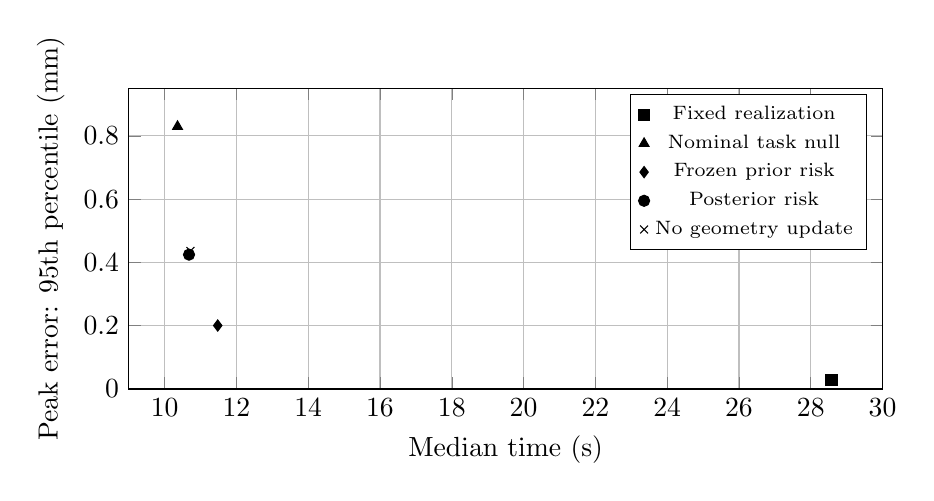
\begin{tikzpicture}
\begin{axis}[width=.92\linewidth,height=5.4cm,xlabel={Median time (s)},ylabel={Peak error: 95th percentile (mm)},xmin=9,xmax=30,ymin=0,ymax=.95,legend style={font=\scriptsize,at={(.98,.98)},anchor=north east},grid=major]
\addplot[only marks,mark=square*] coordinates {(28.580,0.02719)};
\addlegendentry{Fixed realization}
\addplot[only marks,mark=triangle*] coordinates {(10.360,0.82949)};
\addlegendentry{Nominal task null}
\addplot[only marks,mark=diamond*] coordinates {(11.480,0.20044)};
\addlegendentry{Frozen prior risk}
\addplot[only marks,mark=*] coordinates {(10.680,0.42446)};
\addlegendentry{Posterior risk}
\addplot[only marks,mark=x] coordinates {(10.720,0.43598)};
\addlegendentry{No geometry update}
\end{axis}\end{tikzpicture}
\caption{释放任务自由度与后验评价的收益分开。后验方法并非最快或最小误差；它在已声明模型中改善保守方案与名义方案之间的权衡。}
\end{figure}

\subsection{反馈能力变化的敏感性}
主结果之后，补充固定增益 $k_e=1$ 与 $6\,\mathrm{s^{-1}}$ 的敏感性分析，使用独立种子 6104、每组 64 个对象，保留同样的 RMS 预算。它是机制压力测试，不是独立的临床泛化验证。

\begin{table}[ht]\centering\small
\begin{tabular}{lrrr}\toprule
反馈增益 & 名义任务零空间 & 冻结风险 & 后验风险\\\midrule
1.0 & 55/64 & 64/64 & 63/64\\
6.0 & 64/64 & 64/64 & 64/64\\
\bottomrule\end{tabular}
\caption{敏感性实验中曲线全程满足 $1\,\mathrm{mm}$ 误差的运行数。反馈足够强时，名义方法已经可以成功；较弱反馈时后验方法仍不保证零失效。}
\end{table}

较弱反馈下，后验限制减少了任务变形引起的偏移，但仍有失效；冻结风险更保守。较强反馈下，名义方法也全部满足阈值，新增后验主要改变误差幅度而非完成率。该结果支持收益依赖于实际反馈余量，不支持概率模块在所有扫描中都必不可少。

\subsection{八自由度机器人中的局部几何见证}
从固定提交的 URDF 提取全部关节原点、轴、限位及真实 TCP 固定变换。取
\begin{equation}
 q_0=(0.4,0.3,0.6,0.4,1.0,0.2,0.4,0.1)^\top,
 \label{eq:q0}
\end{equation}
第一维单位为米，其余为弧度。以当前声束方向构造深度 $50\,\mathrm{mm}$ 的合成目标和切向，接触面穿过当前 TCP。完整位姿 Jacobian 数值秩为 6，四个扫描等式加接触平面的规则 Jacobian 数值秩为 5。

在相同关节居中代价下比较 60 次局部投影／Newton 回缩：固定 TCP 模式的代价由 $0.078115$ 降到 $0.074523$；允许任务等价变形的代价降到 $0.073463$，TCP 移动 $3.032\,\mathrm{mm}$、姿态改变 $3.471^\circ$，61 个保留节点上的最大归一化规则残差为 $3.78\times10^{-14}$。两条路径均保持采样点关节限位。

进一步让目标深度在 $34,42,50,58,66\,\mathrm{mm}$ 五种假设间变化，三维名义规则零空间内的风险 Gram 只有一个显著正特征值，约 $8.98\times10^{-4}$：两维机械冗余不改变 TCP，新增的一维视角运动则受深度不确定性影响。这是患者后验与任务自由度连接的具体运动学证据。

本测试没有运行 dIRD 网络、真实接触力、碰撞检测或区间连续认证；关节居中代价是可微偏好的替代品。不得把样本残差或局部运动学路径称为真实患者的安全扫查。

\section{先例边界、适用范围与论文门槛}
\label{sec:novelty}
\begin{table}[ht]\centering\small
\begin{tabularx}{\linewidth}{p{.22\linewidth}YY}
\toprule
直接先例 & 已有职责 & V6.1 要建立的具体增量\\\midrule
 iTaSC\cite{itasc} & 任务／不确定坐标、估计与控制统一 & 当前患者后验约束允许变形的整体概率算子\\
 TSR\cite{tsr} & 位姿集合、约束规划及位姿不确定性 & 移动材料任务、局部更新和轨迹偏好的共同执行接口\\
 声窗优化\cite{chatelain} & 保持目标中心声束对齐并优化图像质量 & 不确定规则微分、整族候选查询和机器人能力共同评价\\
 NS-KMP／LC-NS-KMP\cite{nskmp,lcns} & 示教相关性、零空间调制、硬约束与 RL & 零示教规则生成；定义约束的患者几何本身未知\\
 Transportation Maps\cite{transport} & 非线性策略运输及不确定性 & 保持原扫描规则而非仅运输选定标签，并查询当前对象可靠变形\\
 CBTL\cite{cbtl} & 在规划约束剩余自由度中学习偏好 & 接触局部成像、同一解剖场和连续规则段的定量误差接口\\
\bottomrule
\end{tabularx}
\caption{部分文献同时覆盖多个栏目的职责；本表不表示全领域首创性已被证明。}
\end{table}

本次最清楚的方法增量是：\textbf{定义等价性的患者几何也是未知的；同一后验必须既评价目标，又评价允许的动作。}共同规则表示把 dIRD 查询、位姿变化和概率风险放到一个数学对象中，而不是把一个独立预测器接在可达性评分前。

当前证明覆盖声明的静态／时间增广潜模型、可登记目标算子和统一有限步合同。对急剧滑移、未知离散分叉、骨／气体导致的非平滑可见性、严重接触失配或未验收图册，需拒绝原证书并进入相应感知／恢复模式。换器官复用的是规则与算子接口，不是上一患者的后验，也不是所有任务都相同的自由度数。

论文的最终高度需要三类实证：同一允许动作集下优于强确定性任务方法；同样反馈和真实输入下，后验确实改善误差--速度或合格覆盖；另一任务可由相同算子编译而无需重新手工设计估计结构。本轮已给出模型内支持，但真实 dIRD--UltraPoC 执行链尚未完成。因此不能以本稿长度或数值精度宣布 IJRR 全项达到 4 分。

\section{结论}
V6.1 将轨迹从任务定义降为优先实现，并用患者后验决定规则允许的运动在当前证据下能够使用多大幅度。调和坐标保存材料意义，GP／AL-DMP 提供无需人工示教的连续参考，dIRD 利用规则允许的变形优化实现，接触执行层保留其硬限制。新增理论围绕同一规则族的查询闭合、相关性保留和有限段验收组织，不再围绕最小探查预算扩写。核心假设与基线结果同时表明：真正价值来自可靠利用任务自由度，而不来自概率表示本身的复杂程度。

\appendix
\section{规则族闭合与材料几何的证明}
\label{app:closure}
\subsection{条件查询与候选数无关}
在式\eqref{eq:rb} 下，若 $Y=a(\xi)+H(\xi)v$，则对固定数据与候选 $q$，
\begin{equation}
 h=C(q)\widetilde Y,\quad
 \mu_h=C(q)\begin{bmatrix}a+Hm_t\\1\end{bmatrix},\quad
 \Sigma_h=C_Y(q)H C_tH^\top C_Y(q)^\top,
 \label{eq:conditionalquery}
\end{equation}
其中 $C_Y$ 是不含常数列的部分。候选堆叠仅增加确定性矩阵行数。对 $q$ 的任意已存在导数以 $\partial_qC$ 替代 $C$，仍对 $v$ 仿射。对材料相位求导时须将 $\partial_sY$ 预先包括在 $Y$ 中。由此证明定理\ref{thm:closure} 第一项。

令 $\mu_Y(\xi)$、$\Sigma_Y(\xi)$ 为内层矩，则
\begin{equation}
 M_t=\int\left(
 \begin{bmatrix}\Sigma_Y(\xi)&0\\0&0\end{bmatrix}
 +\begin{bmatrix}\mu_Y(\xi)\\1\end{bmatrix}
  \begin{bmatrix}\mu_Y(\xi)\\1\end{bmatrix}^{\!\top}
 \right)\pi_t(\xi)d\xi .
 \label{eq:sharedmoment}
\end{equation}
任意两个规则查询 $h_i=C_i\widetilde Y,h_j=C_j\widetilde Y$ 满足
$\E[h_ih_j^\top]=C_iM_tC_j^\top$，保留了跨候选和跨相位相关性。所有候选在条件于 $\D_t$ 后都是确定的，故无需针对优化结果重新定义患者概率。若原来没有包含某种查询，先扩充生成族、重新检查条件结构，不能因为候选数有限就跳过验收。

更一般地，把所需二次模型写成 $f_\iota(z)=c_\iota+\ell_\iota^\top z+z^\top Q_\iota z$，选 $z=U\xi+Vv$。残余二次项为 $v^\top V^\top Q_\iota Vv$，它对任意 $v$ 消失当且仅当 $V^\top Q_\iota V=0$。这证明 V5.1 条件接口的代数基础。其后高斯观测乘条件高斯先验仍为高斯，外层权重乘边际似然；不能再次把未条件化的先验重复乘入扩维后验。

\subsection{器官位置、导数与面积法向}
写 $Z(u)=h_0(u)+b_\beta(u)+\lambda_\gamma(u)[d_0(u)+B(u)w]$。去掉已知刚体变换，$X=(g_1,g_2,Z)$，则
\begin{equation}
 \partial_1X\times\partial_2X=
 \begin{bmatrix}
 g_{2,1}Z_2-g_{2,2}Z_1\\
 g_{1,2}Z_1-g_{1,1}Z_2\\
 g_{1,1}g_{2,2}-g_{1,2}g_{2,1}
 \end{bmatrix}.
 \label{eq:normalproof}
\end{equation}
因此高度导数的相互乘积抵消，条件于几何伸缩 $\gamma$ 后仍对 $(\beta,w)$ 仿射。已知 $g$ 可包含复杂图册细节，但这些细节只改变系数。若将该面积向量归一化、求随机旋转矩阵，或在未知目标上求非线性切片交点，闭合不再自动成立。

在 $\lambda_\gamma>0$、$g$ 一一可逆时，固定射线模型的逆为 $u=H((R_0^\top(x-p_0))_{1:2})$，随后由第三分量恢复 $d$。Jacobian 行列式为 $\lambda_\gamma\det Dg$。这既说明有效域，也说明站位登记未使用未知深度。它不覆盖未知横向登记误差；该误差需扩充模型。

\subsection{规则实现族的局部维数}
式\eqref{eq:fiber} 是二维表面上的一个正则标量水平集，由隐函数定理局部为一维。$b\perp t$ 使给定 $R$ 正交且右手。联合 $x=(a,q)$ 有十个局部变量，接触点约束一项及 FK 全位姿六项在满秩时共七个独立等式，故维数三。活动不等式可留下切锥而非子空间；接缝、奇异或断开分支需另外处理。此维数计数不证明全程可连接。

\section{风险、相关性和信息变化的证明}
\label{app:freedom}
\subsection{Gram 与精确共同零空间}
将 $A=\bar A+(A-\bar A)$ 代入 $\E[A^\top WA]$，交叉项因条件均值为零消失，得到式\eqref{eq:gap}。对固定 $v$，$v^\top G_tv$ 是非负量 $\norm{A(z)v}_W^2$ 的期望。期望为零当且仅当该量几乎处处为零；$W\succ0$ 给出式\eqref{eq:kernel}。

若 $0<p(\D_t\mid z)<\infty$ 对先验几乎处处成立，则后验与先验具有相同零测集。函数 $A(z)v$ 在一者几乎处处为零当且仅当在另一者成立，因此精确共同零空间不改变。例 $A(\theta)=[1,\theta]$、$\Var(\theta\mid\D_t)>0$ 的 $G_t$ 行列式恰为该方差。任意有限正噪声高斯观测使方差非零，精确秩仍为 2；名义方向 $(-\E\theta,1)$ 的风险则恰为方差。

\subsection{完整残差及忽略相关性的反例}
直接展开 $\E[(r+B\Delta)^\top W(r+B\Delta)]$ 得
\begin{equation}
 \E[r^\top Wr]+2\Delta^\top\E[B^\top Wr]
 +\Delta^\top\E[B^\top WB]\Delta.
 \label{eq:crossproof}
\end{equation}
忽略中间项会改变可行动作，尤其当当前误差与几何 Jacobian 来源于同一潜变量时。即使对每个标量边缘分布都估计正确，破坏联合相关性也不保证保守：$z_1,z_2$ 单位方差、相关系数 $\rho$ 时，$\Var(z_1\pm z_2)=2\pm2\rho$。置零相关性对和低估、对差高估（$\rho>0$）。

\subsection{信息只能在明确意义下降低不确定性}
固定状态和算子，条件期望塔性质直接给出 $\E[G_{t+1}\mid\D_t]=G_t$。将
\[
 A-\bar A_t=(A-\bar A_{t+1})+(\bar A_{t+1}-\bar A_t)
\]
代入 $U_t$，对新历史条件化后交叉项为零，得到式\eqref{eq:uncertaintyreduce}。真实运动到不同状态会改变 $A$，因此不能不加区分地沿实际轨迹套用这个单调关系。

\subsection{为什么不需要识别全部患者参数}
若所有当前需要的规则只通过 $Y=Tz$ 依赖患者参数，则动作评价只需要 $Y$ 的联合后验，无须唯一识别 $\ker T$ 内的变化。例如观察 $z_1+z_2$ 足以确定只依赖该和的任务，即使不能区分两项；任务换成 $z_1-z_2$ 后，旧信息可能不足。这里的充分性针对\emph{声明的查询族}，不是任意未来器官或任意声学异常。

作为简单数据量示例，若只未知深度 $d\sim\N(m_0,s_0^2)$，每帧给独立无偏测量噪声 $\sigma^2$，则 $n$ 帧后
\begin{equation}
 s_n^2=(s_0^{-2}+n\sigma^{-2})^{-1}.
 \label{eq:samples}
\end{equation}
名义居中的侧移--倾斜动作中，若斜率增量为 $\Delta a$，残余方差为 $s_n^2\Delta a^2$。二阶矩阈值 $b^2$ 所需帧数满足
\begin{equation}
 n\ge\left\lceil\sigma^2\left(\frac{\Delta a^2}{b^2}-s_0^{-2}\right)_+\right\rceil.
 \label{eq:sampleillustration}
\end{equation}
这只是已校准独立深度观测的例子，不是本文的主贡献或真实超声通用样本复杂度。有未知公共偏差时方差可存在下限，相关帧不能按独立帧代入。

\section{有限段概率合同与优化器的证明}
\label{app:certificate}
\subsection{定理\ref{thm:segment} 的证明}
记 $a=\epsilon-\rho_t(\Delta x)>0$。在共同有效事件内，式\eqref{eq:remainder} 保证真实规则范数不超过线性预测范数加 $\rho_t$。对任意 $\tau\in[0,1]$，
\begin{equation}
 \norm{r+\tau B\Delta x}_W
 \le(1-\tau)\norm r_W+\tau\norm{r+B\Delta x}_W
 \le\max\{\norm r_W,\norm{r+B\Delta x}_W\}.
\end{equation}
因此整段越过 $\epsilon$ 必须伴随：有效事件失败，或两个仿射端点之一超过 $a$。Markov 不等式给
\[
 \Prob(\norm r_W>a\mid\D_t)\le\frac{\E\norm r_W^2}{a^2}\le\alpha_0,
\quad
 \Prob(\norm{r+B\Delta x}_W>a\mid\D_t)\le\alpha_1.
\]
并集界得到式\eqref{eq:segmentprob}。所有量条件于真实历史，所选动作因而确定；统一余项对该选点同样成立。此证明不要求不同患者假设或各时间段相互独立。

\subsection{数值矩误差与优化后有效性}
若数值 $\widehat\Gamma$ 满足 $\norm{\widehat\Gamma-\Gamma}_2\le\varepsilon_M$，且所有候选 $\norm{\Delta}\le r$，则
\begin{equation}
 [1;\Delta]^\top\Gamma[1;\Delta]
 \le[1;\Delta]^\top\widehat\Gamma[1;\Delta]
      +\varepsilon_M(1+r^2).
 \label{eq:momenterror}
\end{equation}
也可直接使用 $\widehat\Gamma+\varepsilon_MI$ 作 PSD 上界（先验证其对真实矩的上界关系）。这保留二阶锥形式，对全部搜索候选成立。仅在若干选点上的平均积分误差不能代替 $\varepsilon_M$。

dIRD 的平均预测误差同样不能充当硬安全界。它在式\eqref{eq:opt} 中作为目标时，错误主要影响优化收益；只要最终规则和物理验收使用可信模型，接受安全性不依赖其平均精度。若将 dIRD 作为硬约束预测器，则需额外统一代理误差合同。

\subsection{凸性、可行性和递推风险}
$\Gamma\succeq0$ 时存在 $L$ 使 $\Gamma=L^\top L$，故 $\sqrt{\mathcal R(\Delta)}=\norm{L[1;\Delta]}$ 为凸函数；加上 $\sqrt\alpha\rho(\Delta)$ 仍凸。若 $\mathcal K_t$ 是凸集、信赖域凸且目标正定二次，则单次局部问题是凸优化。加入全局分支选择、实际非凸碰撞或非线性声学条件后，应分别搜索／验收，不把局部性质外推。

对失效事件 $E_k$，若 $\Prob(E_k\mid\D_k)\le\alpha_k+\delta_k$，则
$\Prob(\cup_k E_k)\le\E\sum_k\Prob(E_k\mid\D_k)\le\alpha_{\rm total}$。这是条件风险累积；只给每帧相同的 $5\%$ 上界不能推出整次扫描 $5\%$ 风险。随机终止时也必须保持可预测、可求和预算。

\subsection{局部反馈管的替代接口}
若已有接触兼容 servo 在真实系统上满足
\[
 \dot e=-Ke+w_B+w_\Delta,\qquad
 \lambda_{\min}\big((K+K^\top)/2\big)\ge\kappa>0,
\]
则在同一有效域有
\begin{equation}
 \norm{e(t)}\le e^{-\kappa(t-t_0)}\norm{e(t_0)}+
 \int_{t_0}^t e^{-\kappa(t-\tau)}
       \big(\norm{w_B(\tau)}+\norm{w_\Delta(\tau)}\big)d\tau.
 \label{eq:tube}
\end{equation}
可将后验认证的变形扰动界放入该管，协调变形与推进。但当前低层不满足这个模型时，不能仅靠定义 $K$ 继承该结论。本轮扫描机制测试只有 RMS 扰动限制，没有运行完整时变扰动管概率验收。

\section{复现说明、代码范围与审稿式自查}
\label{app:reproduce}
\subsection{文件与执行}
源代码包包含四个运行入口：\texttt{benchmark.py}（概率算子、调和图和主扫描机制）、\texttt{sensitivity.py}（两个反馈增益敏感性）、\texttt{robot\_verify.py}（字面八自由度运动学提取）和 \texttt{reliable\_step.py}（局部凸约束提案及接受检查）。使用 Python、NumPy、SciPy，绘图另需 Matplotlib。示例：
\begin{verbatim}
OPENBLAS_NUM_THREADS=1 OMP_NUM_THREADS=1 python src/benchmark.py --trials 128
OPENBLAS_NUM_THREADS=1 OMP_NUM_THREADS=1 python src/sensitivity.py
OPENBLAS_NUM_THREADS=1 python src/robot_verify.py
OPENBLAS_NUM_THREADS=1 python src/reliable_step.py
xelatex Anatomical_GPS_V6.1.tex
xelatex Anatomical_GPS_V6.1.tex
\end{verbatim}
全部图表数据嵌入本 \texttt{.tex}，单文件编译不依赖额外图片或字体文件；标准 TeX Live 的 Fandol 中文字体足够。源码包不附字体。原始 JSON 和逐次结果用于复核，重跑会因环境产生计时变化。

本轮使用 Python 3.13.5、NumPy 2.3.5；主 1280 次机制运行约 55.6 秒。计时只记录这台共享运行环境，不作为真实控制周期保证。随机种子、分组、输入限值和被排除的空间连接均在代码中显式给出。

运动学来源固定为 RealUS\_playground 提交\par\noindent\path{4766667dad06ba34a38c63790aeb226fef5262ee}。URDF blob 为\par\noindent\path{dddf93c4894aa2c95100da2131282a9b0941b019}。源码包保存的是可检查的运动学参数提取，不声称保存完整 URDF 或网格。参考旧稿是该提交中的 V4.1 和 V5.1；本轮未推送任何 GitHub 修改。

\subsection{为避免再次偏离核心的删减}
正文保留规则、共同查询、可靠动作与执行权衡。V5.1 的最小条件维数证明和历史多项式统计量按已建立接口使用，不重新扩写；V4.4 的探查跨度和最少方向数不进入 V6.1 主贡献。若后续实验证明 ordinary task servo 足以获得相同性能，应缩小概率模块的论文地位，而非新增更多工具维持选题。

\subsection{本轮证据等级与潜力评分}
本轮未调用独立子 agent，也没有外部审稿意见。下表是同一模型从理论、近邻和实现三个角度的自查；不冒充独立 IJRR 分数。
\begin{table}[ht]\centering\small
\begin{tabularx}{\linewidth}{p{.28\linewidth}p{.16\linewidth}Y}
\toprule
维度 & 当前研发判断 & 达到更高评价需要的证据\\\midrule
声明范围内的数学完整性 & 约 $4/5$ & 外部独立证明检查与实现合同验证\\
方法新颖性 & $3.5$--$4/5$ & 相同自由度强基线下，患者后验引起可复现执行差异\\
理论与方法上限 & $4$--$4.5/5$（条件潜力） & 整族算子复用、有限段验收与真实执行成为一个完整方法\\
通用性 & $3.5$--$4/5$ & 第二种真实任务复用相同接口而非重新手写关键模型\\
系统成熟度 & $2.5$--$3/5$ & 实际 dIRD、AL-DMP、UltraPoC、力／碰撞与声窗闭环\\
\bottomrule
\end{tabularx}
\caption{评分不是录用预测；数值残差小不等于原创性高。}
\end{table}

最近的关键反对意见及处理如下。其一，普通任务零空间已经允许 TCP 变形：以同样自由度的名义方法作为强基线，而非只比较锁死 TCP。其二，示教方差调节变形已有 LC-NS-KMP：本文将偏好与定义规则的患者未知量分开，并明确已有工作边界。其三，准确二阶矩不等于连续执行概率：补充完整残差、统一余项和有限段合同，但不将尚未运行的合同归入扫描机制结果。其四，调和图并非独占选择：保留其可复现地址与算子职责，不声称对所有图册最优。其五，八自由度运动学样本并非接触保证：将其与概率和闭环机制结果分别报告。

\subsection{真实系统最小验证协议}
不要求医生示教。优先使用已知内部目标的可变体模，确定实际图像／TCP 标定和保守噪声模型。至少设计一条长曲线与一个多线图块任务；同一参考、同一相位与接触控制器，比较固定实现、名义任务等价、冻结风险和后验风险四种方法。给全部方法相同观测、恢复权限、速度与输入预算；添加声学质量失效时，评分同时保留恢复时间和未完成材料足迹。

预先固定主要指标：合格材料覆盖、峰值与分位成像误差、接触范围、实际输入饱和和完成时间。将每个对象的一次完整运行作为统计单位，不能把相关图像帧当成独立对象。若需要临床效果或跨患者泛化主张，应取得相应真实对象数据及专业审查；本稿不规定可替代这种验证的固定帧数。

\begin{thebibliography}{20}\small
\bibitem{itasc} J. De Schutter et al. Constraint-based Task Specification and Estimation for Sensor-Based Robot Systems in the Presence of Geometric Uncertainty. \emph{IJRR}, 26(5):433--455, 2007. \url{https://doi.org/10.1177/027836490707809107}.
\bibitem{tsr} D. Berenson, S. Srinivasa, J. Kuffner. Task Space Regions: A framework for pose-constrained manipulation planning. \emph{IJRR}, 30(12):1435--1460, 2011. \url{https://doi.org/10.1177/0278364910396389}.
\bibitem{chatelain} P. Chatelain, A. Krupa, N. Navab. Confidence-driven control of an ultrasound probe: Target-specific acoustic window optimization. \emph{ICRA}, 3441--3446, 2016. \url{https://doi.org/10.1109/ICRA.2016.7487522}.
\bibitem{nskmp} J. Silv\'erio, Y. Huang. A Non-parametric Skill Representation with Soft Null Space Projectors for Fast Generalization. \emph{ICRA}, 2988--2994, 2023. \url{https://arxiv.org/abs/2209.08522}.
\bibitem{lcns} A. Padalkar, F. Stulp, G. Neumann, J. Silv\'erio. Towards Safe and Efficient Learning in the Wild: Guiding RL With Constrained Uncertainty-Aware Movement Primitives. \emph{IEEE RA-L}, 10(7):6880--6887, 2025. \url{https://doi.org/10.1109/LRA.2025.3566599}.
\bibitem{transport} G. Franzese, R. Prakash, C. Della Santina, J. Kober. Generalizable Motion Policies through Keypoint Parameterization and Transportation Maps. 用户提供的 2025 年版本，\url{https://arxiv.org/abs/2404.13458}.
\bibitem{cbtl} T. Silver et al. Coloring Between the Lines: Personalization in the Null Space of Planning Constraints. 2025 年预印本，\url{https://arxiv.org/abs/2505.15503}.
\bibitem{kmp} Y. Huang, L. Rozo, J. Silv\'erio, D. G. Caldwell. Kernelized Movement Primitives. 用户提供的期刊论文版本，\url{https://arxiv.org/abs/1708.08638}.
\bibitem{prodmp} G. Li et al. ProDMPs: A Unified Perspective on Dynamic and Probabilistic Movement Primitives. 2022. \url{https://arxiv.org/abs/2210.01531}.
\bibitem{aldmp} T. Ga\v{s}par, B. Nemec, J. Morimoto, A. Ude. Skill learning and action recognition by arc-length dynamic movement primitives. \emph{Robotics and Autonomous Systems}, 100:225--235, 2018. \url{https://doi.org/10.1016/j.robot.2017.11.012}.
\bibitem{floater2003} M. S. Floater. One-to-one piecewise linear mappings over triangulations. \emph{Mathematics of Computation}, 72:685--696, 2003. \url{https://doi.org/10.1090/S0025-5718-02-01466-7}.
\bibitem{floater2006} M. S. Floater, V. Pham-Trong. Convex combination maps over triangulations, tilings, and tetrahedral meshes. \emph{Advances in Computational Mathematics}, 25:347--356, 2006. \url{https://doi.org/10.1007/s10444-004-7620-5}.
\bibitem{murray} L. M. Murray, D. Lund\'en, J. Kudlicka, D. Broman, T. B. Sch\"on. Delayed Sampling and Automatic Rao--Blackwellization of Probabilistic Programs. \emph{AISTATS}, PMLR 84, 2018. \url{https://proceedings.mlr.press/v84/murray18a.html}.
\bibitem{v41} Anatomical GPS V4.1，项目历史工作稿。固定提交 \texttt{4766667d} 的 \path{NMI_idea/ideas/Anatomical_GPS_V4.1.tex}，\url{https://github.com/NingMeng0903/RealUS_playground}。不作为外部已发表论文。
\bibitem{v51} Anatomical GPS V5.1，可编译的材料概率任务基元，项目历史工作稿。同一固定提交的 \path{NMI_idea/ideas/Anatomical_GPS_V5.1.tex}。不作为独立已验证的真实扫描系统。
\end{thebibliography}
\end{document}
